\documentclass[border=10pt]{standalone}

\usepackage{tikz}
\usepackage{tikzsymbols}
\usetikzlibrary{calc,patterns,shapes.geometric}

\def\centerarc[#1](#2)(#3:#4:#5){\draw[#1] ($(#2)+({#5*cos(#3)},{#5*sin(#3)})$) arc (#3:#4:#5);}

\begin{document}
	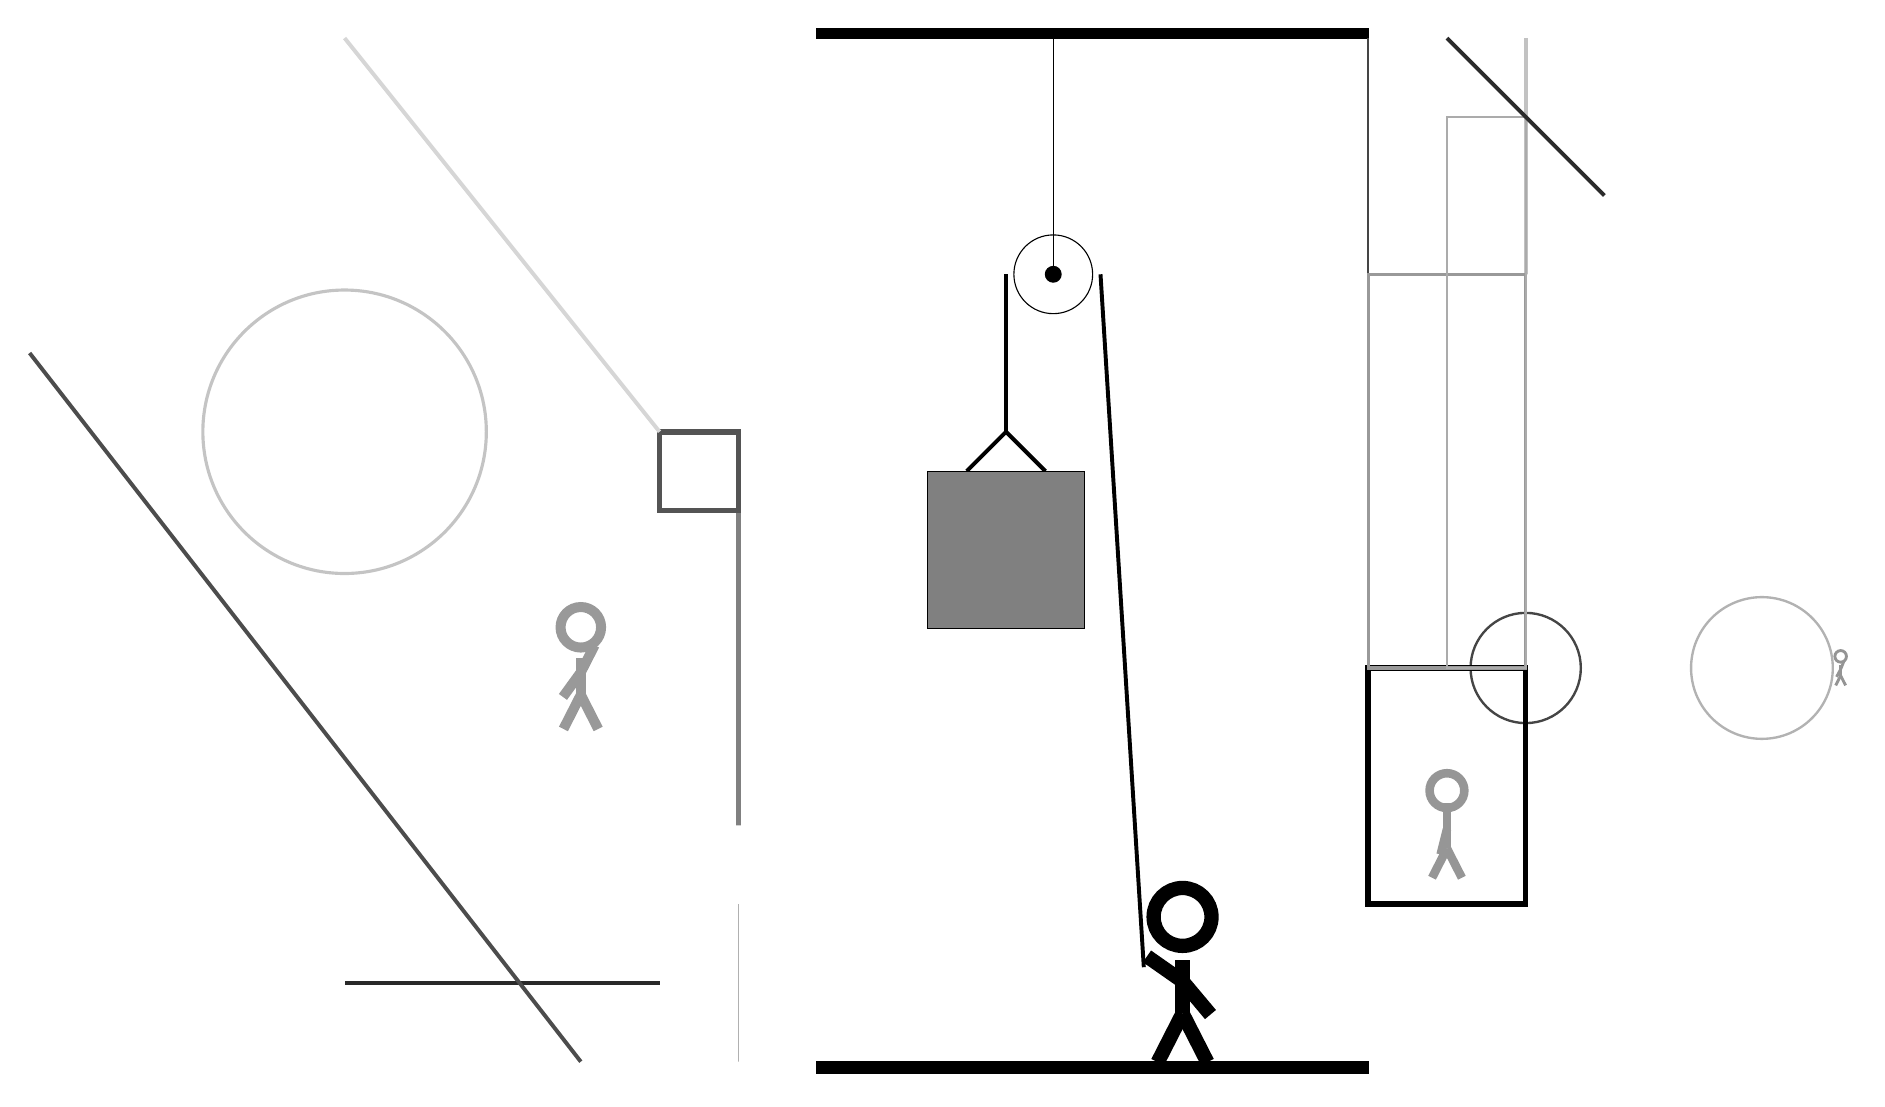
\begin{tikzpicture}
		%%%%% START %%%%%
		
		\draw[fill=black] (-2, 10) rectangle (5, 10.125);
		
		\draw (1, 7) circle (0.5);
		\draw[fill=black] (1, 7) circle (0.1);
		\draw (1, 10) -- (1, 7);
		
		\draw[line width=0.5mm] (-0.1, 4.5) -- (0.4, 5.0) -- (0.9, 4.5);
		\draw[fill=black!50] (-0.6, 4.5) rectangle (1.4, 2.5);
		
		\draw[line width=0.5mm] (0.4, 7) -- (0.4, 5.0);
		\centerarc[line width=0.5mm](1, 7)(0:180:0.6);
		\draw[line width=0.5mm](1.6, 7) -- (2.15, -1.8);
		
		\draw [line width=0.3mm, color=black!73](7, 2) circle (0.7);
		
		\draw[line width=0.3mm, color=black!73] (5, 10) rectangle (5, 6);
		\node[line width=0.4mm, color=black!42] at (11, 2) {\Strichmaxerl[2][62][68]};
		\draw[line width=0.7mm, color=black!100] (7, 2) rectangle (5, -1);
		\draw[line width=0.5mm, color=black!24] (7, 7) rectangle (7, 10);
		\draw[line width=0.4mm, color=black!40] (7, 7) rectangle (5, 2);
		
		\draw [line width=0.4mm, color=black!23](-8, 5) circle (1.8);
		\draw[line width=0.2mm, color=black!33] (7, 9) rectangle (6, 2);
		\draw[line width=0.7mm, color=black!50] (-3, 4) rectangle (-3, 0);
		
		\draw[line width=0.5mm, color=black!84](-4, -2) -- (-8, -2);
		\node[line width=0.7mm, color=black!41] at (6, 0) {\Strichmaxerl[6][76][90]};
		
		\draw[line width=0.7mm, color=black!67] (-3, 4) rectangle (-4, 5);
		\draw[line width=0.5mm, color=black!70](-5, -3) -- (-12, 6);
		
		\draw [line width=0.3mm, color=black!30](10, 2) circle (0.9);
		\node[line width=0.5mm, color=black!40] at (-5, 2) {\Strichmaxerl[7][54][63]};
		\draw[line width=0.5mm, color=black!16](-4, 5) -- (-8, 10);
		\draw[line width=0.2mm, color=black!31] (-3, -1) rectangle (-3, -3);
		\draw[line width=0.5mm, color=black!83](8, 8) -- (6, 10);
		
		\node at (2.6, -1.9) {\Strichmaxerl[10][-35][-50]};
		
		\draw[fill=black] (-2, -3) rectangle (5, -3.15);
		
		%%%%% END %%%%%
	\end{tikzpicture}
\end{document}